\chapter{Data}
\label{kap:data}

Zvukový odkaz Karla Makoně je východiskem pro tuto práci. O jeho
díle neexistuje téměř žádná sekundární literatura, snad kromě článku
v~religionistickém časopise Dingir, viz Hájek (2007)\cite{hajek2007cesky}. Osobně
považuji Makoňovo dílo za jedno z~nejzásadnějších vůbec v~oblasti duchovního
průkopnictví, a to jeho systematičností, obsáhlostí, návodností, novátorstvím a
především hloubkou. Jeho nauka se od moderních duchovních směrů odlišuje kladným
postojem k~civilizačnímim trendům, nikoliv jejich zavrhováním, dále
konzistentním souladem s~rozumovým poznáním a pevnými základy v~náboženských
tradicích. Od vědeckého bádání se odlišuje zejména tím, že rozum a hmotu
považuje za odrazové můstky k~hlubšímu poznání, nikoliv za vrchol a jedinou
platformu lidského poznání. Trvá však na tom, že duchovní zákonitosti jsou
stejně tak pevně dané, univerzální a ověřitelné (ovšem pouze osobní, subjektivní
zkušeností), jako zákony přírodní, popsané vědecky. Do třetice od klasické
křesťanské literatury se liší obzvláště tím, že Ježíšovu nauku považuje za návod
prvotřídní kvality pro vědomý vstup do věčného života zde na zemi a v~těle,
nikoliv po smrti. Věčným životem se míní stav, kdy člověk je vědomě věčnou
bytostí nezávislou na pomíjejícím těle. Tvrdě kritizuje překonaný a naivní
výklad, podle nějž se ctnostným životem dá dojít po smrti do nebe, dále dojít
spásy pouhou proklamací o~víře v~Krista a dodržováním přikázání a náboženských
obřadů.

Odkrývá smysl života a návod na jeho uskutečnění, který nestojí na slepé víře
ani na vlastní omezené lidské invenci.

\section{Karel Makoň}

\subsection{Život Karla Makoně}

Ing. Karel Makoň se narodil 12. prosince 1912. Ve věku dvou let ho postihl zánět
levého ramene. Lékaři doporučovali amputaci ruky, k~čemuž jeho matka nedala
souhlas a na vlastní zodpovědnost nechala dítě operovat. Vzhledem k~tomu, že
ještě nebyly objeveny krevní skupiny, nebyla možná transfúze a proto musela být
operace prováděna opakovaně, aby dítě nevykrvácelo. Tehdejší anestetika nebylo
možné mladému organizmu podávat tak často, proto byly operace prováděny při
vědomí. Malý Karel Makoň se, zažívaje nesnesitelnou bolest, naučil v~raném věku
opouštět při vědomí svoje tělo. Tato opakovaná zkušenost měla u něho následek, že po
určitou dobu nepoznával svoji matku, zato začal spontánně rozpoznávat správné od
nesprávného a důsledně činit, co poznával jako správné.

Pro omezení rizika komplikací s~operovanou rukou bylo Karlovi zakázáno hrát si
s~dětmi. Svůj předškolní čas proto trávil sám na venkově jen se zvířaty. Díky
extrakorporálním zkušenostem se naučil rozumět řeči zvířat, obzvláště hus, které
ho vzaly za svého a s~nimiž pronikal do stavu zvířecího ráje.

Období ,,činění správného``, kdy si kupříkladu zapověděl kouření, alkohol i
veškerý pohlavní život, vyvrcholilo v~Makoňových sedmnácti letech, kdy
narazil na myšlenku, že ,,tento život je mostem do věčnosti``. Tím započalo období
extází a vědomí, že je nesmrtelnou bytostí a smyslem jeho života je spojení
s~Bohem. Svojí matkou a prarodiči byl sice veden ke tradiční katolické víře, ale
nikdy na ni nepřistoupil, protože ,,v~nebi, kde by se jen díval na Boží tvář by
byla strašná nuda``. Nikdy tedy nevěřil, v~sedmnácti letech {\em poznal}.

V~tomto období se ustavičně modlil za to, aby dokázal Boha více milovat. Tato
modlitba trvala devět let a jejím vyvrcholením byla deportace do koncentračního
tábora v~Sachsenhausen v~roce 1939, coby českého vysokoškolského studenta.

V~koncentračním táboře byl Makoň sužován více, než ostatní: měl jakýsi
obzvláštní talent chytat rány a kopance. Prožíval nesmírné zmatení a frustraci
nad tím, že tak dlouho tak věrně sloužil Bohu, a teď se s~ním jedná jako s~kusem
hadru. Po čtyřech dnech utrpení nastal zlomový okamžik. Tamějším vězňům bylo
zakázáno pod trestem smrti přihlížet zabití spoluvězňů příslušníky SS. Makoň si
však nedal pozor a hleděl právě na takovou scénu. Vykonávající Němec si toho
povšiml a vyzval Karla Makoně, ať zůstane stát na místě, že hned, jak dobije
svoji momentální oběť, přijde zabít i jeho. Karel Makoň v~tu chvíli raději
odevzdal svůj život Bohu, a to bez přemýšlení a bezpodmínečně, se silou nabytou
onou devítiletou modlitbou. Překvapivým výsledkem toho bylo, že SS-Mann tváří
v~tvář Makoňovi zbledl a v~hrůze se obrátil na útěk.

Makoň tehdy obdržel všeobjímající poznání smyslu života
a absolutní svobodu. Pohyboval se volně od baráku k~baráku, nezažíval hlad ani
jiný nedostatek, esesáci jako by ho neviděli. Trávil svoje dny v~koncentračním táboře
burcováním ostatních k~probuzení k~pravdě, kterou sám zažíval.

Zanedlouho byl z~koncentračního tábora propuštěn. Celý zbytek svého života
věnoval předávání svojí zkušenosti a hlavně návodu, jak k~takové zkušenosti
přijít bez nutnosti zažívat extáze i dramatické krize, neboť obojí považuje za
nepříkladné.

Zemřel v~roce 1993.

\subsection{Spisovatelská a přednášková činnost}

Již roku 1936 napsal Karel Makoň dopis {\em Utrpení a láska}, který poslal na
podporu trpícímu příteli. Roku 1939 přeložil spis {\em Bhakti
jóga}\cite{vivekananda2003bhakti} od významného indického filozofa Svámího  Vivékánandy.
Jeho pozdější práce už rozvíjejí jeho vlastní dosažené poznání.

Do roku 1992, kdy v~činnosti ustal, napsal a přeložil dílo o celkovém rozsahu
3~613~211 slov nebo též 25~069~991 znaků, čili necelých 14 tisíc normostran.
Nejrozsáhlejším jeho dílem je trilogie {\em Mystika}, která sestává z~dílů
\begin{enumerate}
\item{{\em Západní starověká tradice}  (1948),}
\item{
    {\em Srovnání jógy s~křesťanskou mystikou}
    (1986--1989) obsahující překlad děl
    {\em Syntéza jógy}\cite{aurobindo1999synthesis} od indického filozofa Šrí
    Aurobinda Ghóše
    a {\em Hrad nitra}\cite{teresa1588castillo} od středovéké křesťanské
    mystičky sv. Terezie z~Avily,
}
    \item{{\em Výklad evangelia Sv. Jana} (1950--1953).}
\end{enumerate}

Dalšími rozsáhlými knihami jsou {\em Cesta vědomí} (1973--1974),
dále výklad církevního roku a církví doporučených biblických čtení
{\em Postila} (1965),
{\em Sladké jho} (1977--1980) obsahující překlad části díla
{\em Précis de Théologie Ascétique et Mystique}\cite{tanquerey1928precis}
od francouzského teologa Adolphe-Alfreda Tanquerey,
{\em Umění následovat Krista} (1971),
autobiografické {\em Umění žít} (1969)
a {\em Základní kurs nadživotnosti pro ty, kteří si myslí, že nevěří a základní
kurs náboženství pro ty, kteří si myslí, že věří, neboť jsou si všichni rovni,
pokud umírají, aniž by se během života znovu narodili} (1967--1968).

Nikoliv rozsahem, ale významem jsou hodny zmínky spisy
{\em Oběť mše svaté} (1951), kde je účast na katolické liturgii podána jako
návod pro spojení s~věčností,
{\em Pohádka na dobrou noc} (1980), kde je odhalen duchovní smysl pohádky o
Honzovi
a {\em Blahoslavenství} (1973).

Makoňovo dílo se šířilo převážně samizdatem, a to i po
Sametové revoluci. Psané dílo bylo několikrát kompletně přepsáno na
psacích strojích a po příchodu osobních počítačů ještě jednou. Všechny knihy a
spisy jsou volně k~dispozici na stránkách \texttt{makon.cz}. Jen hrstka knih
byla vydána, a sice
\begin{enumerate}
\item{Umění následovat Krista (1992)\cite{makon1995umeni},}
\item{
    Pohádky nejen pro děti (1992 pod názvem {\em Odkrytá moudrost starých
    pravd}) \cite{makon1992odkryta},
}
\item{Utrpení a láska (1995)\cite{makon1995utrpeni},}
\item{
    Mystická koncentrace (1995 pod názvem
    {\em Mystická koncentrace a příprava k~ní})\cite{makon1995mysticka},
}
\item{
    Otázky a odpovědi I - IV (1999 pod názvem {\em Světlo na cestu})\cite{makon1999svetlo},
}
\item{
    Blahoslavenství
    (2000)\cite{makon2000blahoslavenstvi}\footnote{\label{note1}
        Duchovní úlohy a Blahoslavenství mají, zdá se, totožné ISBN.
    },
}
\item{
    Úlohy (2002 pod názvem {\em Duchovní
    úlohy})\cite{makon2002ulohy}\footnotemark[\getrefnumber{note1}],
}
\item{Základní kurs nadživotnosti (2005)\cite{makon2005zakladni}.}
\end{enumerate}

Většina děl se snaží podat více či méně ucelený návod pro vědomý vstup do
věčnosti, vždy z~jiného východiska nebo pro jiný typ čtenáře. Například {\em Umění
žít} je věnováno Makoňově nejmladší dceři a je z~velké části vlastním
životopisem. {\em Základní kurs nadživotnosti, pro ty, kteří si myslí, že nevěří, a
základní kurs náboženství pro ty, kteří si myslí, že věří,} je kniha, která má
společný úvod a závěr, ale hlavní stať je rozdělena na dvě oddělené části, jednu
pro lidi nevěřící v~Boha, kde se autor opírá o experimenty s~tělem a o kritický
přístup, zatímco v~druhé části důkladně rozebírá smysl Otčenáše a radí,
jak tuto modlitbu praktikovat pro její spojovací účel. {\em Umění následovat
Krista} se zase soustředí na systematizaci cesty v~rozdělení na očistnou,
osvěcovací a spojovací část, jak to vykládá křesťanská mystická tradice.

\subsection{Rysy Makoňovy nauky}

Pokusím se krátce představit charakteristiky Makoňovy nauky,
jak je hodnotím podle svojí osobní zkušenosti a svého
názoru. Serióznější porovnání by bylo námětem na jinou disertaci na jiné
fakultě.

Karel Makoň je moderním učitelem duchovní moudrosti. Jako mnozí vychází z~křesťanství. Považuje Bibli za vrcholný zdroj
moudrosti a Ježíšův život a výroky za nejdokonalejší návod k~duchovní realizaci,
jaký je nám momentálně k~dispozici. Zdůrazňuje, že je vždy potřeba se řídit
Ježíšovým příkladem jako celkem, nikdy částí vytrženou z~kontextu. Každý Ježíšův
výrok a úkon má svůj protiklad. Jednou například Ježíš hlásá nenásilí a radí
,,nastavit druhou tvář``, ale podruhé bičem vyhání kupce z chrámu. Jedině syntéza výroků a činů s~jejich protiklady
mohou podle Makoně poskytnout použitelný návod, kterým se dá v~životě obecně
řídit.

Striktně zavrhuje doslovný výklad tzv. nadpřirozených událostí. Například
apokalypsa -- konec světa a druhý příchod Ježíšův, je podle něho ryze individuální záležitostí, která se
stane každému člověku v~jiný okamžik podle jeho vývoje. Dokládá to Ježíšovým
výrokem, že ,,nepomine toto pokolení, než se to všecko stane`` (Mk 13,30), dále
srovnáním s~fenoménem mystické smrti, známým od mnoha jednotlivců i různých
tradic, a vlastní zkušeností. Stejně tak stvoření světa je podle něho popisem
vývoje lidského jedince, obzvlášť jeho nitra. K~tomu zdůrazňuje, že nejde o
jednorázový čin, nýbrž soustavné tvoření, které neustále probíhá, a
sedm dní stvoření je sedm kvalit, které jsou ve stvoření neustále přítomny.

Rozlišuje mezi Ježíšem, který symbolizuje naši věčnou podstatu, a Kristem, který
symbolizuje spasitelský úkol Boží. Že tento není závislý na fyzické osobě Ježíše,
dokládá jeho výrokem: ,,Dříve, než Abraham byl, já jsem.`` (J 8,58)

Karel Makoň má několik oblíbených pasáží z~Bible, ke kterým se často vrací. Asi
nejvýznamnějšími z~nich je podobenství o marnotratném synu a podobenství o
hřivnách. V~podobenství o marnotratném synu (Lk 15,11-32) popisuje symbol plně rozvinutého
lidského života, kde promrhání znamená investici do pomíjejícího, a je nezbytnou
podmínkou pro vzpomínku na otcův dům, tedy uvědomění si vlastní věčné podstaty, a
sjednocení bytosti kolem touhy po návratu. Otcovo ocenění syna šatem, prstenem a
zabitím telete ukazuje na fakt, že jde o vyšší a tedy žádoucí stav oproti
,,dobrému synovi``, který otcovo dědictví nepromarnil. Podobenství o hřivnách (Lk 19,11-27)
předestírá jako návod pro životní situace obecně, kde se doporučuje spatřovat
nejen ve statcích, ale i v~situacích hřivny dané od Boha, se kterými nakládáme
nikoliv pro sebe, ale pro něho. Zúčtování, kdy hospodář přichází, aby si vzal
výtěžek z~hřiven, máme vidět v situacích, kdy přicházíme o kontrolu nad
výsledkem svého snažení či nad situací. Moment odevzdání hřiven hospodáři bez
sebemenší pohnutky nechat si z~výtěžku něco pro sebe je klíčovým a následné udělení měst
namísto hřiven k~hospodaření je univerzálním pravidlem rozmnožení darů a
zodpovědnosti.

Křesťanské tradici vyčítá operování s~nevyzpytatelnou Boží milostí. Bůh podle
Karla Makoně není člověk a tím méně náladový člověk, aby se mu tu něco zlíbilo a
ondy nezlíbilo nebo znelíbilo. I města za hřivny v~podobenství obdrželi služebníci nikoliv na
základě toho, jakou měl hospodář náladu, nýbrž podle míry svého hospodaření.
Stejně tak je zákonité, kdy člověka potká mystická zkušenost a vůbec cokoliv, co
tradice připisuje nevyzpytatelné Boží milosti. Podmínky pro tuto dispozici
důkladně popisuje. Já jen shrnu, že stěžejním bodem je, jak to vyplývá
z~podobenství o hřivnách, vynaložení veškerých lidských sil (znásobení hřiven
bez přítomnosti hospodáře) pro nadpozemský cíl (hospodaření pro hospodáře, ne
pro sebe) a následné dokonalé odevzdání, když jsou lidské síly vyčerpány.

Dalším výrazným rysem Makoňovy nauky je, že vše podřizuje dosažení království
Božího, čímž se odlišuje od mnoha moderních duchovních učitelů, kteří mnohdy
vycházejí z~lidských potřeb šťastného života, vztahů, hojnosti a podobně. Jednak
ho to připodobňuje ke klasickým katolickým autorům a jednak (podle mne právě
proto) jeho nauka zaujme jen nepatrný zlomek lidí, kteří mají zájem o duchovno.
Světské lidské problémy nebagatelizuje, doporučuje naopak univerzální metodu pro
jejich řešení, například v~díle {\em Zlatý klíč}, ale pro člověka,
který nehledá království Boží především, je tato metoda v~podstatě nepřístupná.

Na rozdíl od většiny moderních učitelů moudrosti má Karel Makoň velmi pozitivní
postoj ke všem civilizačním změnám, včetně technizace, rozmachu
všudypřítomného vlivu systému, daním atp. Považuje je za příležitost nežít pro
sebe, nýbrž pro společnost, a tím trénovat život pro věčnost. Naopak vůči
sexualitě, sám užívaje termín ,,pohlavní život``, se staví mnohem zdrženlivěji,
než většina mně známých moderních autorů. Vidí v~sexualitě především vybíjení
boží síly za účelem vstupu do zvířecího ráje a doporučuje aspoň část života
prožít bezpohlavně.

\section{Témata v mluveném korpusu}

Celý mluvený korpus Karla Makoně, jakož i jeho celé psané dílo, má jednotné
téma, jež by se dalo shrnout jako návod k~vědomému spojení s~věčností.
V~průběhu času i podle toho, komu byla konkrétní promluva určena, se však mění 
i témata jemnějšího rozlišení.

Můžeme nalézt témata opakující se napříč celým korpusem.
Namátkou mohu zmínit:

\begin{enumerate}
\item{soupeření Eliáše s Bálovými kněžími,}
\item{stvoření jako probíhající proces,}
\item{Job,}

\item{otcovství Josefovo,}
\item{přivolení Mariino,}
\item{události po Ježíšově narození,}
\item{prvních 30 let Ježíšova života,}
\item{křest v~Jordánu,}
\item{zázrak na svatbě v~Káně galilejské,}
\item{podobenství o marnotratném synu,}
\item{podobenství o hřivnách,}
\item{blahoslavenství,}
\item{spící Ježíš na rozbouřeném moři,}
\item{symbolika apoštolů coby lidských schopností,}
\item{Máří Magdaléna,}
\item{Lazar,}
\item{úkol Jidášův,}
\item{lotr na kříži,}
\item{ukřižování,}

\item{obrácení Šavla ve svatého Pavla,}
\item{manželé, kteří padli mrtvi, ve Skutcích,}

\item{Svatá Terezie z~Avily,}
\item{Otec Pio,}
\item{Svatý František z Assisi,}
\item{Svatá Terezie z Lisieux,}
\item{Svatý Augustin,}

\item{Lao C´,}
\item{Milarepa,}
\item{Siddhárta Gautama Buddha,}
\item{Rámakrišna,}
\item{Karel Weinfurter,}

\item{operace v~dětství,}
\item{život se zvířaty,}
\item{extatické stavy,}
\item{neschopnost hřešit,}
\item{konání správného,}
\item{devět let modlitby a skrytá sebeláska,}
\item{koncentrační tábor,}
\item{operace ledvin,}
\item{vlité poznání,}

\item{opuštění dosaženého stupně,}
\item{krize na cestě,}
\item{celobytostné sjednocení,}
\item{sebeodevzdání,}
\item{číselná symbolika v~Kabale,}
\item{symbolika rakety,}
\item{symbolika matematických vzorců,}
\item{úloha neklidu,}
\item{první krok na cestě,}
\item{pohádka o Honzovi,}
\item{posmrtný život,}
\item{hadí síla,}
\item{Satan,}
\item{čakramy,}
\item{pohlavní život,}
\item{stylizace života,}
\item{zákonitost Boží milosti,}
\item{sat, čit, ánanda,}
\item{indická tradice,}
\item{Tao,}
\item{mithraismus.}

\end{enumerate}

Jmenovaná témata můžeme rozdělit do následujících kategorií
\begin{itemize}
\item{starozákonní postavy a události,}
\item{život Ježíšův,}
\item{ostatní postavy a události Nového zákona,}
\item{křesťanští světci,}
\item{ostatní významné osobnosti,}
\item{události z~Makoňova vlastního života}
\item{prvky na cestě k~Bohu obecně.}
\end{itemize}

Systematická
identifikace témat a anotace korpusu vzhledem k~nim je předmětem budoucí práce.
Inspirací pro tematickou anotaci může být např. Skorkovská (2011)\cite{skorkovska2011automatic}.


O zmapování témat a jejich pokrytí v~korpusu proběhlo a probíhá několik pokusů.
Prvním z~nich jsou strojově psané indexy k~magnetofonovým
páskám. Ty jsem nafotil do 258 fotografií, pro ilustraci viz
obrázek~\ref{fig:index-kotouc}. Jejich obsahem je posloupnost
záznamů, z~nichž každý je uvozen pozicí počítadla na magnetofonu, za čímž
následuje shrnutí tématu přibližně do 50 znaků. Některé záznamy jsou zvýrazněny
podtržením či kapitálkami. Typická délka jednoho takto označeného úseku je 1--10
minut. Tyto indexy jsou přiložené k~nahrávkám. Problémem je, že u kotoučů
není patrné, který digitalizovaný soubor odpovídá které stopě označené v~indexu
jako {\em a}, {\em b}, {\em c} nebo {\em d}.

\begin{figure}[htpb]
\includegraphics[scale=0.192]{rc/index-kotouc.jpg}
\caption{Index přiložený k~jednomu z~kotoučů.}
\label{fig:index-kotouc}
\end{figure}

Krom toho existují podrobnější indexy ve formě listů
formátu A4, psané z~menší části na stroji, z~větší části psacím písmem, kde
interval mezi jednotlivými úseky je často v řádu desítek sekund. Těch je
nafocených 350 stran. Viz příklad na obrázku~\ref{fig:index-rucni}.

\begin{figure}[htpb]
\includegraphics[scale=0.95]{rc/index-rucni.jpg}
\caption{Ručně psaný index.}
\label{fig:index-rucni}
\end{figure}

V~rámci tohoto projektu učinil Ing. Milan Tulach vždy po přepisu přednášky výběr
pasáží, které považoval za stěžejní, a opatřil je časovými značkami.
Pokryl tak toho času 44 nahrávky.

K~poslouchaným nahrávkám si dělám poznámky stejným způsobem jako jsou k~ručně psaným
indexům, ale digitálně a pozice označuji identifikátorem
nahrávky a časovou pozicí. Zatím jsem takto pořídil 2626 záznamů ze~170 nahrávek.

Pozice počítadla magnetofonu v indexech
jsem se pokusil převést na časové údaje. Počítadlo se inkrementuje při každé
otáčce cívky, na kterou se páska navíjí. Uplynulý čas je tedy kvadratická funkce
pozice počítadla. Mělo by tedy stačit nalézt několik málo odpovídajících párů
pozic počítadla a času a z~toho interpolovat koeficienty v~hledaném polynomu.

Tak jsem dospěl k~výrazu $t = 0,0008605c^2 + 1,674c + 3,998$. Bohužel vyšlo
najevo, že po hodině trvání nahrávky se kotouč otáčí tak pomalu, že pozice
počítadla se změní až za několik desítek sekund. To způsobuje, že interpolační
koeficienty jsou velmi nepřesné a v~kombinaci s~nepřesností při určování nové
pozice to způsobuje, že začátek hledaného tématu se nachází i více než minutu
před či za predikovanou pozicí.

Tento problém lze řešit buď přesnějším určením funkce času podle pozice
počítadla, a to použitím hardwarového počítadla či přesnější interpolací
pomocí většího množství bodů, anebo využitím predikce začátku
tématu v~několikaminutovém okolí pomocí komputačnělingvistických metod.

\section{Nahrávání}
\label{sec:data:rec}

O průběhu nahrávání mám pouze kusé a anekdotické informace. Nejstarší datum, na
které jsem u nahrávky narazil, je z~roku 1970. Je možné, že některé nahrávky
jsou staršího data, ale nic nenasvědčuje tomu, že by jich bylo mnoho a byly
výrazně starší. Vzhledem k~tomu, že Karel Makoň začal evangelizovat už
v~koncentračním táboře na konci roku 1939 a přestal až v~roce 1992, je
pravděpodobné, že záznam je k~méně než polovině slov, která vyřkl.

Přednášky v~úzkém kruhu přátel se konaly na různých místech Československa,
později ČR.
Existovala skupinka v~Plzni, v~Praze a v~Gottwaldově, dnešním
Zlíně. Některé z~nahrávek jsou
z~několikadenních skupinových setkání v Kalech u Brna, na chatě Čeřínek v
Českomoravské vrchovině nebo ve Žiaru na Slovensku. Ostatní pocházejí většinou
z~přátelských setkání u někoho v soukromí.

Naprostou většinu nahrávek, které mám k~dispozici, pořídil dr. Elger.
Nahrávalo se s~tehdejší nejmodernější technikou a pásky byly pečlivě
skladovány. Nahrávky z~ostatních míst
také existují, ale jsou spíše raritou a často jsou hůře zachované a ne tak
systematicky označené.

Část nahrávek (30\% celkové délky) je nahraných na kotouče, zbytek na kazety. Ve
většině případů má každý kotouč a každá kazeta identifikátor. Některé kusy
jsou bez identifikátoru, některé dvojice mají totožný identifikátor a různý
obsah.

Většina nahrávek je z~kazet s~identifikátorem ve formátu \texttt{YY-NN}.
Například \texttt{85-05} je pátá kazeta z~roku 1985. Z~takto označených kazet
pochází 686 výsledných souborů z celkových 802, které mají původ v~kazetách.

Celkem z~39 kotoučů, které jsem sám digitalizoval, jich 36 bylo nahraných
rychlostí 9,53 centimetru za sekundu. Zbylé tři rychlostí 2,38 centimetru za sekundu. Na jeden
průchod takového kotouče se vejde šest hodin záznamu, ale za cenu citelného
snížení kvality, zvláště po dekádách skladování. 24 kotouče jsou označeny
písmenem. Posloupnost je více méně abecední, ačkoliv tři různé kotouče sdílejí
identifikátor s~písmenem ,,I`` a nedostala se ke mně žádná páska s~písmenem
,,G``; asi se ztratila. 85 kotoučů (včetně těch, které jsem nedigitalizoval já)
má v~identifikátoru ročník v~rozmezí od 1973 do 1988. Vyskytuje se zde však
mnoho duplicit, takže skutečný počet rozličných nahrávek je v~této kategorii
pravděpodobně mnohem menší. Deset kotoučů má číselný identifikátor, dvacet devět
textový a dva byly vůbec bez identifikátoru.

Existují také dva videozáznamy. Jeden, tříhodinový, je ke zhlédnutí na YouTube:
\texttt{https://www.youtube.com/watch?v=UaNm9jnnJiA}

\section{Digitalizace}
\label{sec:data:digitisation}

U většiny kazet byla digitalizace prováděna stylem jedna strana do jednoho
souboru. U kotoučů to byl jeden kanál jednoho průchodu z~kotouče na kotouč do
jednoho souboru. Výjimku zde tvoří kazety digitalizované v~módu auto-reverse,
s~čímž jsem v~průběhu dvou let digitalizace experimentoval.

Následuje vyčerpávající výčet médií, které odpovídají jednotlivým
digitalizovaným souborům:

\begin{itemize}
\item{strany kazet: 615 souborů,}
\item{celé kazety: 140 souborů,}
\item{průchody z~kotouče na kotouč: 112 souborů,}
\item{převzaté, nejisté: 222 soubory,}
\item{dvě po sobě jdoucí kazety: 1 soubor.}
\end{itemize}

Převzaté soubory byly digitalizovány dříve, než jsem se k~nim dostal. Formát pro digitalizaci, který jsem používal, byl
nejdříve 44100Hz pro prvních 810 souborů, posléze 48kHz,
16 bitů v~reálném čase. Výjimku z~digitalizace v~reálném čase tvoří
kotouče nahrané rychlostí 2,38 cm/s. Ty byly digitalizovány standardní
rychlostí 9,53 cm/s, načež jim byla nastavena čtvrtinová vzorkovací
frekvence.

Pro digitalizaci jsem používal nejdříve zařízení {\em Ion Tape 2 PC}, které
poskytuje USB rozhraní jako externí zvuková karta. Později jsem začal používat
přehrávač {\em Denon DRW-585} a externí zvukovou kartu {\em Lexicon Alpha} coby převodník
z~analogového signálu do digitálního formátu. Kotouče jsem digitalizoval pomocí
přehrávače {\em Tesla B-115} připojeného zezačátku do {\em Ion Tape 2 PC},
později do {\em Lexicon Alpha}.

\subsection{Volba identifikátorů}

Každý takto zdigitalizovaný soubor jsem pojmenoval podle následujícího
algoritmu: Pokud šlo o kazetu s~identifikátorem, použil jsem tento identifikátor
a k~němu připojil písmeno \texttt{A} nebo \texttt{B} pro rozlišení strany. Pokud
byl na obalu nějaký další popisek, připojil jsem ho za pomlčku k~oběma stranám.
Pokud byl popisek na kazetě, připojil jsem ho pouze k~souboru odpovídající strany.

V~případě
kotoučů jsem identifikátor prefigoval řetězcem \texttt{kotouc-} a připojil
rozlišovací dvoumístné číslo počínaje \texttt{01} a označení stopy \texttt{-a}
až \texttt{-d}.

Písmeno \texttt{a} dostal vždy levý kanál prvního průchodu, \texttt{c} pravý
kanál. Písmeno \texttt{b} dostal levý kanál zpátečního průchodu a \texttt{d}
pravý kanál. Ukazuje se, že toto značení nebylo nejšťastněji zvolené, protože
některé kotouče jsem dostal převinuté na opačnou stranu, takže dochází
k~nepředvídatelné záměně mezi písmeny \texttt{a}, \texttt{c} versus \texttt{b},
\texttt{d}.

Pokud nahrávka identifikátor neměla, použil jsem řetězec \texttt{neident} a
pořadové číslo.

\subsection{Přepisy}

K~6. květnu 2020 existuje ke korpusu kompletní přepis o 7 510 610
slovech, z~nichž 715 285, tedy 9,52\% je přepsáno ručně.
Ruční přepisy pokrývají přesně 107 hodin 41 minutu a 49 sekund z~celkových
1050 hodin 5 minut a 3 sekund nahrávek.

První manuálně přepsaný segment byl pořízen v~dubnu 2012 a od té doby do dneška
jich bylo posláno 128 038. Z~toho 113 846, to jest 89\%, pochází od čtyř
přispěvatelů (mezi něž já nepatřím).
Obrázek~\ref{fig:corpus-growth} ukazuje, jak přibývaly hodiny přepisů v~čase.
Počítá se zde celkový objem příspěvků, které se namnoze překrývají, takže
skutečný čas přepsaného záznamu je ,,jen`` zmiňovaných 107 hodin.

\begin{figure}[htpb]
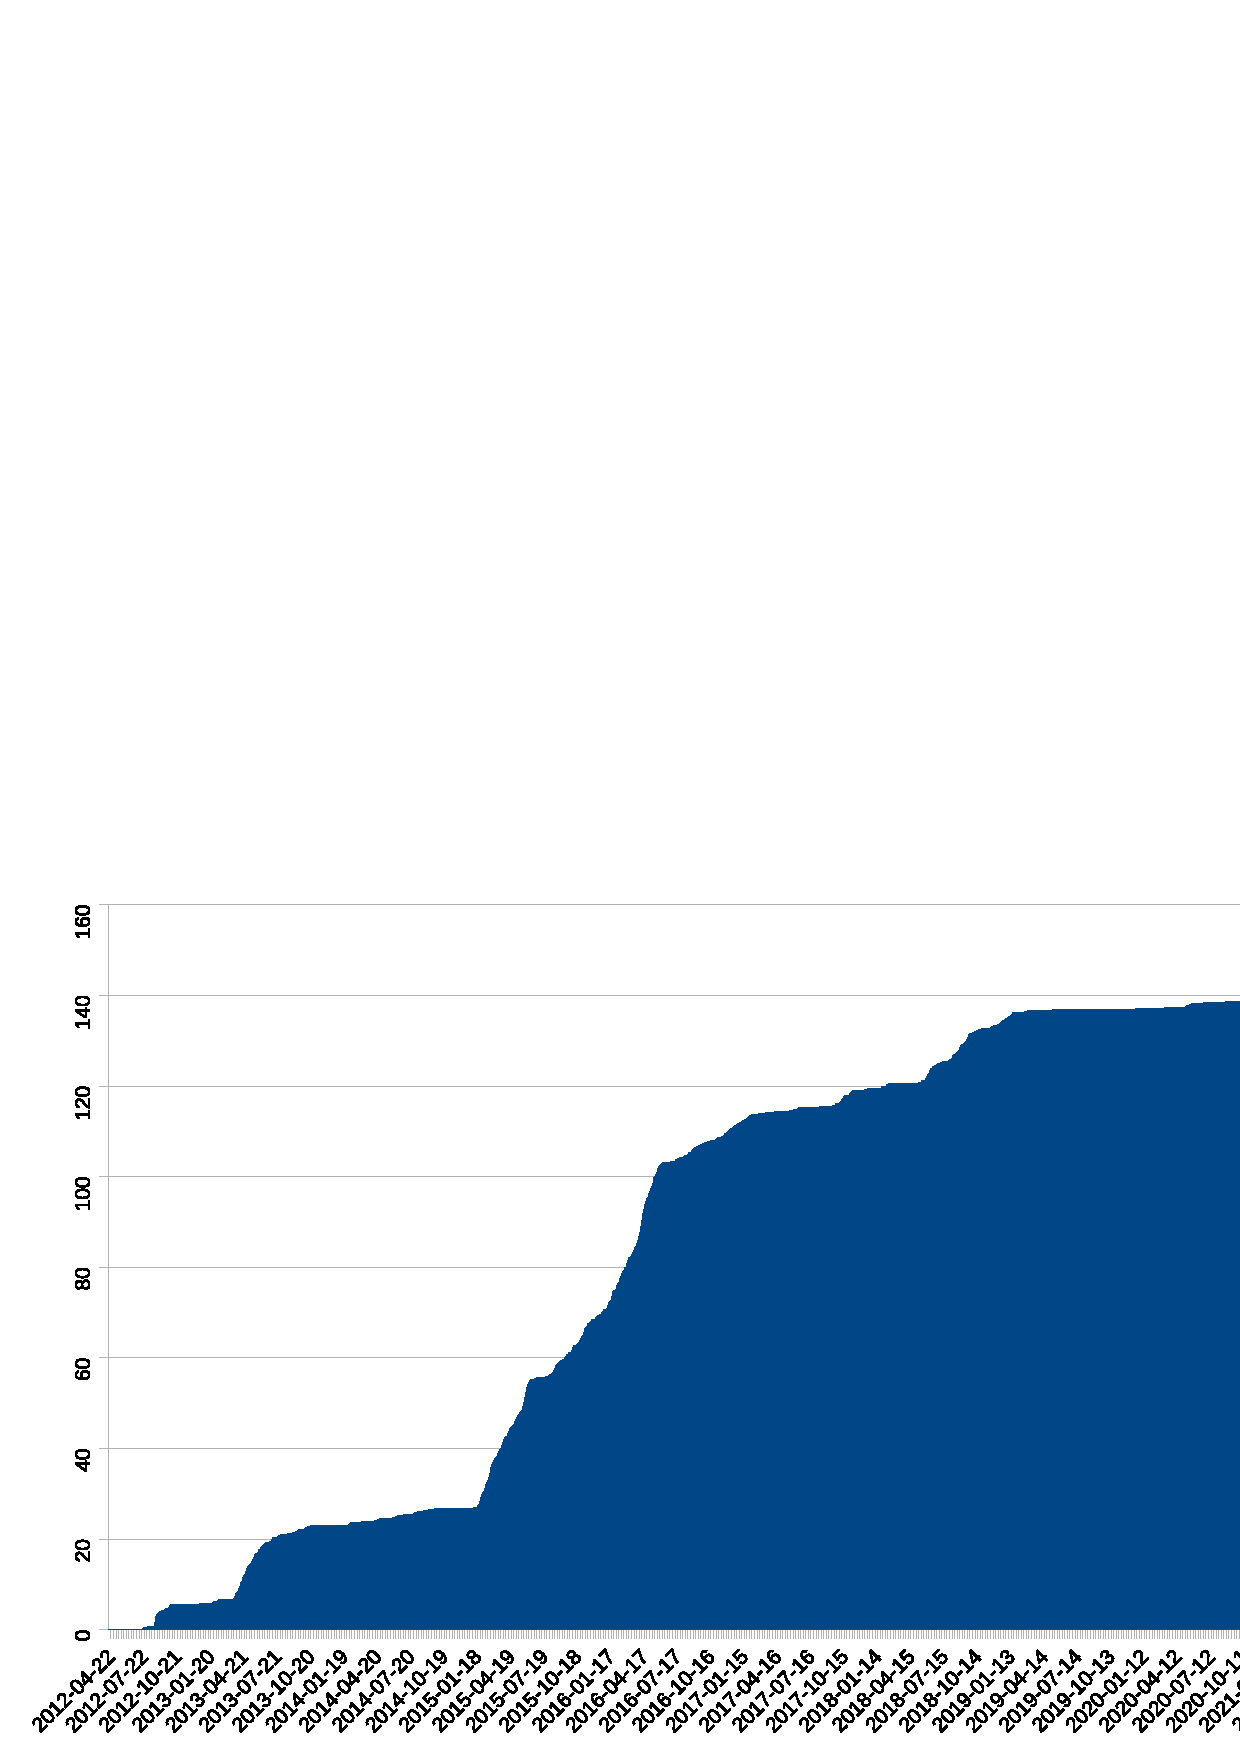
\includegraphics[scale=0.36]{rc/corpus-growth.png}
\caption{Přibývání celkového času oprav.}
\label{fig:corpus-growth}
\end{figure}

Podíl manuálně a automaticky přepsaných pasáží ilustruje
obrázek~\ref{fig:humbits}. Každý pixel reprezentuje jedno slovo v~přepisu,
přičemž černé pixely představují manuálně přepsaná slova.

\begin{figure}[htpb]
\includegraphics[scale=0.137]{rc/humbits.png}
\caption{Distribuce automaticky (bílá) a manuálně (černá) pořízených přepisů.}
\label{fig:humbits}
\end{figure}

Mechanismus pořizování přepisů dopodrobna rozvádí kapitola~\ref{kap:webove-rozhrani}. 
